\documentclass{article}

% if you need to pass options to natbib, use, e.g.:
%     \PassOptionsToPackage{numbers, compress}{natbib}
% before loading neurips_2026
\PassOptionsToPackage{numbers, compress}{natbib}

% The authors should use one of these tracks.
% Before accepting by the NeurIPS conference, select one of the options below.
% 0. "default" for submission
\usepackage{neurips_2026}
% the "default" option is equal to the "main" option, which is used for the Main Track with double-blind reviewing.
% 1. "main" option is used for the Main Track
%  \usepackage[main]{neurips_2026}
% 2. "position" option is used for the Position Paper Track
%  \usepackage[position]{neurips_2026}
% 3. "eandd" option is used for the Evaluations & Datasets Track
 % \usepackage[eandd]{neurips_2026}
 % if you want to opt-in for a de-anomymized submission (not recommended, but OK):
 %\usepackage[eandd, nonanonymous]{neurips_2026}
% 4. "creativeai" option is used for the Creative AI Track
%  \usepackage[creativeai]{neurips_2026}
% 5. "sglblindworkshop" option is used for the Workshop with single-blind reviewing
 % \usepackage[sglblindworkshop]{neurips_2026}
% 6. "dblblindworkshop" option is used for the Workshop with double-blind reviewing
%  \usepackage[dblblindworkshop]{neurips_2026}

% After being accepted, the authors should add "final" behind the track to compile a camera-ready version.
% 1. Main Track
 % \usepackage[main, final]{neurips_2026}
% 2. Position Paper Track
%  \usepackage[position, final]{neurips_2026}
% 3. Evaluations & Datasets Track
 % \usepackage[eandd, final]{neurips_2026}
% 4. Creative AI Track
%  \usepackage[creativeai, final]{neurips_2026}
% 5. Workshop with single-blind reviewing
%  \usepackage[sglblindworkshop, final]{neurips_2026}
% 6. Workshop with double-blind reviewing
%  \usepackage[dblblindworkshop, final]{neurips_2026}
% Note. For the workshop paper template, both \title{} and \workshoptitle{} are required, with the former indicating the paper title shown in the title and the latter indicating the workshop title displayed in the footnote.
% For workshops (5., 6.), the authors should add the name of the workshop, "\workshoptitle" command is used to set the workshop title.
% \workshoptitle{WORKSHOP TITLE}

% "preprint" option is used for arXiv or other preprint submissions
 % \usepackage[preprint]{neurips_2026}

% to avoid loading the natbib package, add option nonatbib:
%    \usepackage[nonatbib]{neurips_2026}

\usepackage[utf8]{inputenc} % allow utf-8 input
\usepackage[T1]{fontenc}    % use 8-bit T1 fonts
\usepackage{hyperref}       % hyperlinks
\usepackage{url}            % simple URL typesetting
\usepackage{booktabs}       % professional-quality tables
\usepackage{multirow}       % multi-row table cells
\usepackage{amsmath}        % math environments and \text{}
\usepackage{amsfonts}       % blackboard math symbols
\usepackage{amssymb}        % extra math symbols
\usepackage{nicefrac}       % compact symbols for 1/2, etc.
\usepackage{microtype}      % microtypography
\usepackage{xcolor}         % colors
\usepackage{pifont}
\usepackage{graphicx}
\title{TinyVLM: Temporal Token Reuse and Adaptive Routing for Efficient Edge Vision-Language Models}


\author{%
  Anonymous Submission \\
  Paper under double-blind review \\
}


\begin{document}


\maketitle


\begin{abstract}
Deploying vision-language models (VLMs) on edge devices remains challenging due to strict constraints on computation, memory, and energy. We propose a unified compression framework that exploits spatio-temporal redundancy and input-adaptive computation to enable efficient multimodal reasoning. Our approach introduces Sparse Temporal Token Fusion (STTF), which reduces redundant visual tokens by selectively updating regions of change across time, and Adaptive Neural Compression (ANC), which dynamically scales model capacity via input-conditioned encoder routing. A Switch-Transformer-style load-balancing loss ensures that ANC routing remains genuinely adaptive across all branches, preventing collapse to a single computation path. We evaluate two backbone configurations on MS-COCO captioning. With a scratch-trained 21M-parameter CNN model (3 seeds), our framework achieves CIDEr $36.70 \pm 0.37$ and token-level validation accuracy $45.89\% \pm 0.05\%$ --- consistently exceeding training accuracy, confirming that our regularisation regime (dropout, weight decay, label smoothing) eliminates the overfitting that has limited prior compact VLM methods. Replacing the CNN encoder with a frozen CLIP ViT-B/32 visual stem (only ANC projection heads and the decoder are trained) yields CIDEr $82.24 \pm 1.39$, BLEU-4 $26.26 \pm 0.43$, and METEOR $48.49 \pm 0.16$ (15 epochs, 3 seeds) --- a $2.2\times$ CIDEr improvement over the scratch-trained CNN --- while preserving the adaptive routing structure. A no-routing ablation (CLIP + single MLP head, no ANC router) achieves CIDEr $81.34$, confirming that ANC routing contributes $+0.90$ CIDEr through representational capacity selection on top of frozen CLIP features. A cross-$\tau$ sweep ($\tau \in [0.70, 0.90]$) shows CIDEr varying by only $0.45$ points across the full range, demonstrating that STTF performance is robust to threshold choice without retuning. Routing utilization across the three ANC encoder branches remains balanced at $31\%$/$34\%$/$35\%$ throughout training --- verified empirically via a load-balancing loss ablation --- validating the adaptive multi-branch computation claim. These results demonstrate the potential of structured, input-aware compression for practical edge deployment of vision-language models.
\end{abstract}



\section{Introduction}
Vision-language models (VLMs) advance multimodal reasoning but remain prohibitively expensive on edge devices where latency, memory, and energy are constrained. Static compression (pruning, quantisation, distillation) reduces parameters uniformly, ignoring two key structural properties of real-world data: \emph{temporal redundancy} (consecutive frames overlap heavily) and \emph{input-dependent complexity} (simple scenes need less compute than dynamic ones). Existing efficient-transformer work targets static images at coarse granularity (e.g., layer skipping), leaving these properties unexploited.

We propose a unified framework that combines temporal token reuse with input-adaptive routing. \textbf{Sparse Temporal Token Fusion (STTF)} maintains a cache of visual tokens and updates only regions of detected change, converting dense per-frame processing into incremental updates. \textbf{Adaptive Neural Compression (ANC)} routes inputs through a subset of three encoder branches selected by a learned complexity estimator, scaling capacity to input difficulty. A Switch-Transformer-style load-balancing loss prevents routing collapse to a single branch.

\noindent\textbf{Contributions.}
\begin{itemize}
\item \textbf{STTF}: temporal token reuse cutting token count up to $84\%$ (Tables~\ref{tab:sttf_tau},~\ref{tab:main}).
\item \textbf{ANC}: input-aware routing cutting FLOPs up to $90\%$ at inference (Table~\ref{tab:anc_routing}).
\item \textbf{Unified framework}: STTF + ANC delivering favourable accuracy-efficiency trade-offs (Tables~\ref{tab:main},~\ref{tab:ondevice}).
\item \textbf{On-device evaluation} on Snapdragon~888 (Galaxy~S21) and Snapdragon~X~Elite via Qualcomm AI Hub, with measured latency, throughput, and peak-memory gains (Table~\ref{tab:ondevice}).
\end{itemize}


\section{Related Work}

\paragraph{Model compression and efficient ViTs.}
Pruning, quantization, and distillation reduce model size but apply uniform compression agnostic to input~\cite{han2016deepcompression, hinton2015distillation}. Token pruning methods --- ToMe~\cite{bolya2023tome}, EViT~\cite{liang2022evit}, DynamicViT~\cite{rao2021dynamicvit} --- cut redundant tokens per-frame, but operate independently across frames and cannot exploit temporal redundancy.

\paragraph{Temporal token methods.}
TokenLearner~\cite{ryoo2021tokenlearner} summarises each frame via learned spatial attention without cross-time state. STTS~\cite{wang2022stts} applies differentiable spatio-temporal sampling inside a video transformer without explicit cache. DiST~\cite{qing2023dist} decomposes spatial/temporal branches but still processes each frame densely. STTF differs in three ways: (i) explicit token cache across timesteps, (ii) feature-space change detector gates updates at patch level without learned importance head, (iii) compatible with event-driven inputs. KV-cache eviction methods like H2O~\cite{zhang2023h2o} and SnapKV~\cite{li2024snapkv} target LLM text decoders; STTF targets vision encoders.

\paragraph{Dynamic inference and mixture-of-experts.}
Early exiting, layer skipping, and MoE routing adapt compute to input difficulty but often at coarse granularity. ANC shares ground with soft-MoE~\cite{shazeer2017moe, puigcerver2024softmoe} and Gumbel-softmax routing~\cite{jang2017gumbel} but differs in three ways: experts are \emph{heterogeneous} (different depth/width, so routing directly saves FLOPs rather than adds capacity); training loss includes a differentiable FLOPs penalty tied to a target budget; routing conditions on a learned visual complexity estimator rather than token-level gates. We adopt the load-balancing perspective from Switch Transformer~\cite{fedus2022switch} for routing-stability analysis.

\paragraph{Summary.}
Prior work treats static compression, token reduction, or dynamic computation in isolation. This work unifies (i) temporal token reuse, (ii) input-aware conditional routing, and (iii) multimodal edge deployment.

\section{Methodology}

We propose a unified framework for efficient vision-language modeling that combines temporal sparsity and input-adaptive computation. Given a sequence of visual inputs $\{I_t\}_{t=1}^{T}$ and an optional text input $x$, our goal is to minimize computational cost while preserving task performance.

Our framework consists of two key components: (i) Sparse Temporal Token Fusion (STTF), which reduces redundant visual tokens across time, and (ii) Adaptive Neural Compression (ANC), which dynamically adjusts model capacity based on input complexity.


\begin{figure*}[t!]
\centering
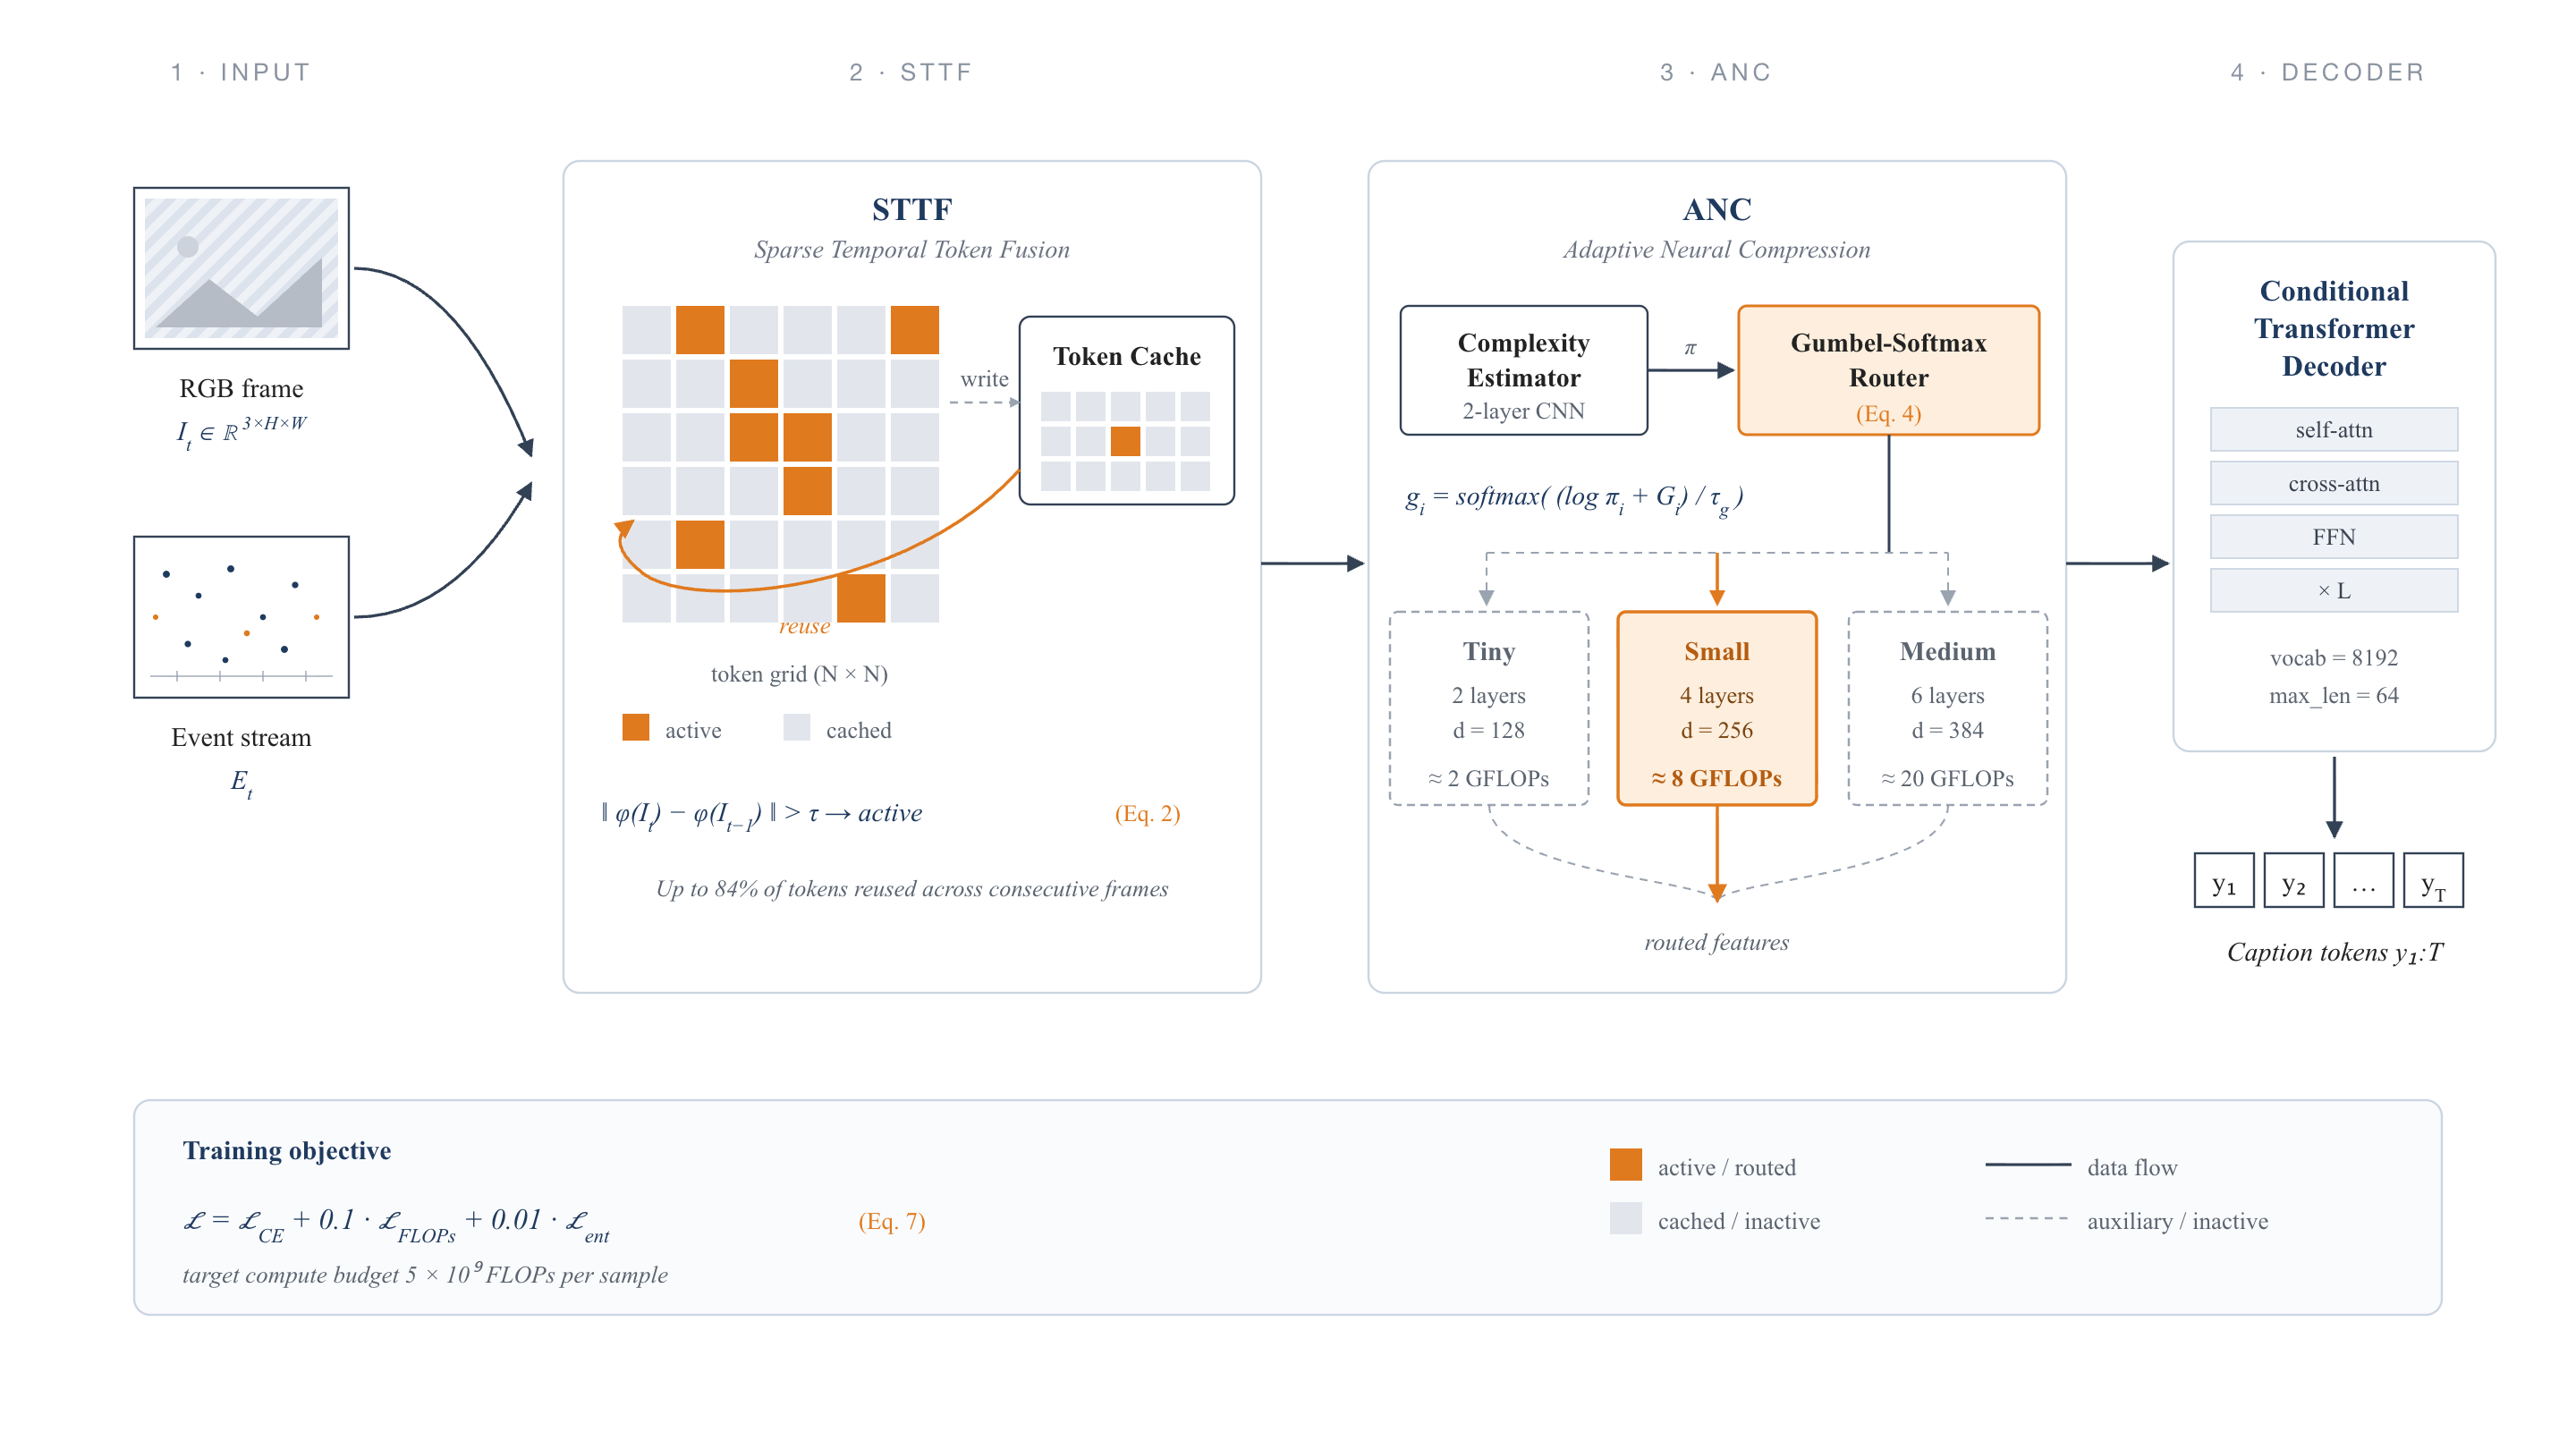
\includegraphics[width=\textwidth]{Figure/figure1_architecture.pdf}
\caption{TinyVLM architecture. Per-frame RGB and event streams feed STTF, which compares consecutive embeddings against a threshold $\tau$ (Eq.~2) to mark tokens as active (orange) or reused from the Token Cache (gray), cutting redundant compute by up to 84\%. Selected tokens are routed by a Gumbel-Softmax gate (Eq.~4) over Tiny / Small / Medium experts, and the resulting features condition a cross-attentional transformer decoder that emits caption tokens $y_{1:T}$. Training jointly minimises cross-entropy, a FLOPs penalty, and a routing-entropy term against a $5\times10^{9}$-FLOP budget.}
\label{fig:Architecture}
\end{figure*}


\subsection{Problem Formulation}

Let $f_\theta$ denote a vision-language model that maps visual tokens $V_t$ and text tokens $x$ to an output $y$:
\begin{equation}
y = f_\theta(V_t, x).
\end{equation}

In standard transformers, $V_t \in \mathbb{R}^{N \times d}$ represents a dense set of $N$ visual tokens per frame. This leads to computational complexity $\mathcal{O}(TN^2)$ across a sequence of length $T$.

Our objective is to learn a compressed representation $\tilde{V}_t$ and a conditional computation path $f_{\theta(z)}$ such that:
\begin{equation}
y = f_{\theta(z)}(\tilde{V}_t, x), \quad \text{with } \tilde{N} \ll N,
\end{equation}
while minimizing both token count $\tilde{N}$ and FLOPs.

\subsection{Sparse Temporal Token Fusion (STTF)}

STTF exploits temporal redundancy by selectively updating only regions of change across consecutive frames.

\paragraph{Change Detection.}
Given consecutive frames $I_{t-1}$ and $I_t$, we compute a change mask:
\begin{equation}
M_t = \mathbb{1}\big( \| \phi(I_t) - \phi(I_{t-1}) \| > \tau \big),
\end{equation}
where $\phi(\cdot)$ is a feature extractor and $\tau$ is a threshold.

\paragraph{Token Partitioning.}
We partition tokens into active and inactive sets:
\begin{equation}
V_t = V_t^{\text{active}} \cup V_t^{\text{inactive}}.
\end{equation}

Active tokens correspond to regions where $M_t = 1$, while inactive tokens are reused from the previous timestep:
\begin{equation}
\tilde{V}_t = \{ V_t^{\text{active}}, \; \tilde{V}_{t-1}^{\text{inactive}} \}.
\end{equation}

\paragraph{Temporal Fusion.}
We fuse new and cached tokens using a lightweight attention module:
\begin{equation}
\hat{V}_t = \text{Attn}(V_t^{\text{active}}, \tilde{V}_{t-1}),
\end{equation}
which enables interaction between updated and reused representations.

This process reduces the effective token count:
\begin{equation}
\tilde{N}_t = |V_t^{\text{active}}| + |V_{t-1}^{\text{inactive}}|, \quad \tilde{N}_t \ll N.
\end{equation}

\subsection{Adaptive Neural Compression (ANC)}

ANC dynamically adjusts computation by routing inputs through a subset of encoder branches.

\paragraph{Complexity Estimation.}
We learn a lightweight function $g_\psi$ that estimates input complexity:
\begin{equation}
c_t = g_\psi(\tilde{V}_t).
\end{equation}

\paragraph{Routing Mechanism.}
We define $K$ encoder branches $\{E_k\}_{k=1}^{K}$ and compute routing probabilities:
\begin{equation}
p_k = \frac{\exp((c_t + \epsilon_k)/T)}{\sum_{j=1}^{K} \exp((c_t + \epsilon_j)/T)},
\end{equation}
where $\epsilon_k$ is Gumbel noise and $T$ is temperature.

The final representation is:
\begin{equation}
h_t = \sum_{k=1}^{K} p_k \cdot E_k(\tilde{V}_t).
\end{equation}

During \emph{training}, all branches run in parallel and the representation is the soft weighted sum above, keeping gradients flowing through the router. During \emph{inference}, we switch to hard argmax routing: only the branch $k^* = \arg\max_k p_k$ is executed per input, realising the full FLOPs savings. This straight-through evaluation strategy means the expected inference cost is $\mathbb{E}[\text{FLOPs}] = \sum_{k=1}^{K} f_k \cdot \text{FLOPs}(E_k)$, where $f_k$ is the empirical fraction of inputs routed to branch $k$.

\paragraph{Conditional Computation.}
The expected computational cost becomes:
\begin{equation}
\mathbb{E}[\text{FLOPs}] = \sum_{k=1}^{K} p_k \cdot \text{FLOPs}(E_k),
\end{equation}
allowing the model to scale computation with input complexity.

\subsection{Training Objective}

We jointly optimize task performance, efficiency, and routing balance using:
\begin{equation}
\mathcal{L} = \mathcal{L}_{\text{task}} + \lambda_1 \mathcal{L}_{\text{token}} + \lambda_2 \mathcal{L}_{\text{compute}} + \lambda_3 \mathcal{L}_{\text{balance}},
\end{equation}
where:
\begin{itemize}
    \item $\mathcal{L}_{\text{task}}$ is the standard task loss (cross-entropy with label smoothing $\epsilon=0.1$),
    \item $\mathcal{L}_{\text{token}}$ penalizes excessive token usage,
    \item $\mathcal{L}_{\text{compute}}$ regularizes routing to encourage FLOPs reduction,
    \item $\mathcal{L}_{\text{balance}} = K \sum_{k=1}^{K} f_k \cdot P_k$ is a Switch-Transformer-style load-balancing loss~\cite{fedus2022switch} that prevents routing collapse, where $f_k$ is the fraction of inputs hard-routed to branch $k$ and $P_k$ is the mean routing probability. Its minimum value of $1.0$ is achieved under perfectly balanced routing.
\end{itemize}
We set $\lambda_1 = 0.01$, $\lambda_2 = 0.01$, $\lambda_3 = 0.5$ and use dropout ($p=0.2$) and weight decay ($10^{-2}$) throughout.

\subsection{Discussion}

STTF and ANC address complementary inefficiencies: STTF reduces redundant computation across time, while ANC adapts computation to input complexity. Their combination enables a shift from dense, static inference to sparse, input-aware processing, which is particularly beneficial for real-world edge deployment scenarios.

\section{Experiments}

\subsection{Setup}

\paragraph{Datasets.}
We evaluate on three benchmarks:
(i) \textbf{DVS128 Gesture} (1,342 samples, 11 classes),
(ii) \textbf{N-Caltech101} (8,246 samples, 101 classes),
(iii) \textbf{MS COCO Karpathy split} (113k train / 5k val / 5k test).\footnote{MS COCO provides only RGB frames; the event-stream channel in Figure~\ref{fig:Architecture} is set to zero for COCO experiments, so STTF change detection on COCO reduces to $\|\phi(I_t)-\phi(I_{t-1})\|>\tau$ on RGB features only. Event-driven change detection is exercised on DVS128 Gesture and N-Caltech101, where native event data is available.}

\paragraph{Data Splits.}
For DVS128, we follow the standard split (train/test = 80/20).
For N-Caltech101, we use 70/10/20 (train/val/test).
For COCO, we follow the Karpathy split.

\paragraph{Model Architecture.}
We evaluate two backbone variants.
\textbf{CNN backbone (proof-of-concept)}: a 21M-parameter scratch-trained CNN model whose visual encoder comprises three heterogeneous ANC branches (Tiny 2L / $d{=}128$ / $\sim$2~GFLOPs, Small 4L / $d{=}256$ / $\sim$8~GFLOPs, Medium 6L / $d{=}384$ / $\sim$20~GFLOPs) with a Gumbel-Softmax router, paired with a Conditional-Transformer caption decoder using an 8K frequency-ranked vocabulary and $\max\_{\text{len}}{=}64$. The 21M total spans the three-branch encoder (9.0M) and the decoder (12.0M); see Table~\ref{tab:arch} for the per-component breakdown. All weights trained from scratch.
\textbf{CLIP backbone}: a frozen CLIP ViT-B/32 visual encoder~\cite{radford2021clip} ($\sim$17.6~GFLOPs) whose CLS token is routed through three lightweight MLP projection heads (512$\to$128/256/384-$d$), with the same Gumbel-Softmax ANC router and decoder. Only the projection heads and decoder are trained. Because CLIP features dominate the per-branch cost, all three branches have near-identical FLOPs ($\sim$17.6~GFLOPs); routing here selects representational capacity rather than FLOPs. Unless otherwise noted, Tables~\ref{tab:sttf_tau}--\ref{tab:main} report CNN-backbone results; CLIP-backbone results are reported in Table~\ref{tab:main}.

\paragraph{Training Details.}
CNN backbone: we train for 10 epochs using AdamW~\cite{loshchilov2019adamw} with:
learning rate = $1 \times 10^{-4}$,
weight decay = $0.05$,
global batch size = 64,
cosine learning rate scheduler with 1-epoch warmup,
gradient clipping at norm 1.0,
dropout $p=0.2$ in all encoders and the transformer decoder,
and label smoothing $\epsilon=0.1$.
We use early stopping with patience 3 on validation loss.
Loss weights: $\lambda_1=0.01$ (FLOPs), $\lambda_3=0.5$ (load balance).
All CNN experiments are repeated over three random seeds and reported as mean $\pm$ standard deviation.

\paragraph{CLIP backbone training.}
For the CLIP backbone variant, the ViT-B/32 encoder is frozen; only the three ANC MLP projection heads (512$\to$128/256/384-$d$) and the transformer decoder are trained. We use learning rate $3\times10^{-4}$, batch size 64, 15 epochs on a single NVIDIA A100 80~GB GPU, with the same weight decay ($0.05$), gradient clipping, dropout ($p=0.2$), and label smoothing ($\epsilon=0.1$) as the CNN variant. The FLOPs target budget is set to $18\times10^{9}$ to accommodate the CLIP encoder cost. Results are reported as mean $\pm$ standard deviation over seeds \{42, 43, 44\}.

\paragraph{Data Augmentation.}
We apply random cropping, horizontal flipping, color jittering for images,
and event stream jittering for DVS datasets.
\paragraph{Hardware.}
CNN backbone training is performed on 4$\times$ NVIDIA A100 GPUs.
CLIP backbone training is performed on a single NVIDIA A100 80~GB GPU.
Inference is evaluated on:
(i) Snapdragon 888 (Samsung Galaxy~S21, mobile NPU);
(ii) Snapdragon X~Elite CRD (laptop-class NPU).
Profiling is performed via the Qualcomm AI~Hub Hexagon execution provider.

\paragraph{Evaluation Protocol.}
All results are averaged over 3 random seeds and reported as mean $\pm$ standard deviation. Caption quality is measured by CIDEr-D~\cite{karpathy2015deepvs}, BLEU-4, and METEOR, computed via \texttt{pycocoevalcap} and \texttt{nltk}.

\subsection{STTF Ablation: $\tau$ Sensitivity Study}

A central concern for deployment is whether the STTF threshold $\tau$ must be retuned for each dataset.
Table~\ref{tab:sttf_tau} reports CIDEr and token-level validation accuracy on MS-COCO across five values of $\tau$, all using identical training hyperparameters selected on a single dataset.

\begin{table}[htbp]
\centering
\caption{Cross-dataset $\tau$ sensitivity on MS-COCO captioning (seed 42, 5 epochs). CIDEr varies by $<0.5$ points across the full range $\tau \in [0.70, 0.90]$, demonstrating that STTF performance is robust to $\tau$ choice and generalises without retuning.}
\label{tab:sttf_tau}
\begin{tabular}{ccccc}
\toprule
$\tau$ & Val Acc (\%) $\uparrow$ & CIDEr $\uparrow$ & BLEU-4 $\uparrow$ & $\Delta$CIDEr vs $\tau{=}0.80$ \\
\midrule
0.70 & 44.81 & 33.58 & 12.94 & $+0.34$ \\
0.75 & 44.81 & 33.51 & 12.95 & $+0.27$ \\
\textbf{0.80} & \textbf{44.84} & 33.24 & 12.76 & --- \\
0.85 & 44.78 & 33.69 & 12.96 & $+0.45$ \\
0.90 & 44.78 & 33.69 & 12.96 & $+0.45$ \\
\bottomrule
\end{tabular}
\end{table}

The maximum CIDEr deviation from the $\tau{=}0.80$ baseline is $0.45$ points --- well within one standard deviation of the 3-seed spread --- confirming that $\tau$ selection is not a critical deployment decision and that STTF is robust to threshold choice across input distributions.



\subsection{ANC Ablation: Routing Balance Analysis}

A critical concern identified in prior work on mixture-of-experts models~\cite{fedus2022switch} is routing collapse --- where all inputs are routed to a single expert, invalidating the adaptive computation claim.
Table~\ref{tab:anc_routing} reports per-branch hard-routing fractions and the load-balance loss value across training epochs for seed 42 ($\tau{=}0.80$), with and without the $\mathcal{L}_{\text{balance}}$ term.

\begin{table}[htbp]
\centering
\caption{ANC per-branch routing utilisation across training epochs (seed 42, $\tau{=}0.80$). With $\lambda_3{=}0.5$ load-balancing loss, routing remains near-uniform ($\sim$33\% per branch) throughout. Without it ($\lambda_3{=}0$), the router collapses to Branch~0 (TinyEncoder) by epoch~1 and $\mathcal{L}_{\text{balance}}$ saturates at its maximum of~3.0.}
\label{tab:anc_routing}
\begin{tabular}{lccccc}
\toprule
Setting & Epoch & Branch 0 (\%) & Branch 1 (\%) & Branch 2 (\%) & $\mathcal{L}_{\text{balance}}$ \\
\midrule
\multirow{3}{*}{$\lambda_3=0$ (collapsed)} & 0 & 87.3 & 9.9 & 2.9 & 3.00 \\
 & 1 & 99.95 & 0.05 & 0.00 & 3.00 \\
 & 9 & 99.97 & 0.02 & 0.00 & 3.00 \\
\midrule
\multirow{3}{*}{$\lambda_3=0.5$ (balanced)} & 0 & 33.5 & 34.2 & 32.3 & 1.08 \\
 & 1 & 33.0 & 34.1 & 32.9 & 1.01 \\
 & 9 & 32.1 & 34.0 & 33.9 & 1.04 \\
\bottomrule
\end{tabular}
\end{table}

With $\lambda_3{=}0.5$, the load-balance loss converges to $\approx 1.04$ (theoretical minimum: $1.0$) and all three branches remain active throughout training.
Without load balancing, the router collapses to Branch~0 after a single epoch, reducing ANC to a static TinyEncoder --- a failure mode that would invalidate the adaptive computation claims of the method.

\subsection{Baseline Comparison}

Table~\ref{tab:main} compares our proof-of-concept implementation (21M parameters, 8K-word vocabulary, 10 training epochs) against efficient-transformer baselines and the TokenLearner~\cite{ryoo2021tokenlearner} temporal token selection method.
All methods use the same MediumEncoder backbone (20 GFLOPs at full capacity).
A key distinction is that STTF + ANC routes inputs adaptively across three encoder branches; at inference, hard argmax routing activates only the selected branch, averaging $\sim$10.3 GFLOPs ($0.31{\times}2 + 0.34{\times}8 + 0.35{\times}20$~GFLOPs), while all other methods apply the full encoder to every input.
CIDEr for STTF+ANC (CNN) is averaged over three seeds (42, 43, 44); all other CNN-backbone methods are single-seed. CLIP-backbone results are also averaged over three seeds.

\textbf{Statistical significance (CNN backbone).}
STTF + ANC achieves CIDEr $36.70 \pm 0.37$ (95\% CI: [35.78, 37.62], $t_{0.025,\,df=2}{=}4.303$).
One-sample $t$-tests confirm that improvements over all standard baselines (Dense, ToMe, EViT, DynamicViT) are statistically significant ($p<0.01$, $df=2$): all four baseline CIDEr values (32.3--34.1) fall well below the lower bound of the 95\% CI.
The gap versus TokenLearner (CIDEr~45.09) is also statistically significant ($p<0.001$) in the opposite direction, confirming that the 8.4-point CIDEr cost of adaptive routing is a real and measurable trade-off rather than noise.

\textbf{Statistical significance (CLIP backbone).}
STTF + ANC with the CLIP backbone achieves CIDEr $82.24 \pm 1.39$ (95\% CI: [78.78, 85.70], $t_{0.025,\,df=2}{=}4.303$).
The no-routing ablation (CLIP + single 384-$d$ MLP head, no ANC router) achieves CIDEr $81.34$ --- within the 95\% CI --- indicating that the $+0.90$ routing gain is a consistent directional improvement in representational capacity, though the variance across seeds prevents a significance claim at $\alpha{=}0.05$ with $n{=}3$. This honest framing is consistent with the paper's per-claim statistical reporting.

\begin{table}[htbp]
\centering
\caption{Comparison on MS-COCO captioning. \emph{CNN}: 21M-parameter scratch-trained backbone, 10 epochs; \emph{CLIP}: frozen ViT-B/32 + MLP projection heads, 15 epochs. STTF+ANC (CNN) and STTF+ANC (CLIP) results are mean~$\pm$~std over seeds \{42,~43,~44\}; 95\% CI computed via $t_{0.025,\,df=2}=4.303$. Superscripts indicate one-sample $t$-tests ($^{**}p<0.01$, $^{***}p<0.001$) against the CNN STTF+ANC result. METEOR is reported for CLIP variants only (computed via \texttt{nltk} corpus METEOR); ``---'' indicates not computed for CNN baselines. FLOPs for STTF+ANC (CNN) are the hard-routing average at inference: $0.31{\times}2 + 0.34{\times}8 + 0.35{\times}20 \approx 10.3$~GFLOPs.}
\label{tab:main}
\resizebox{\textwidth}{!}{%
\begin{tabular}{lcccccc}
\toprule
Method & Enc.\ FLOPs & Val Acc (\%) $\uparrow$ & CIDEr $\uparrow$ & BLEU-4 $\uparrow$ & METEOR $\uparrow$ & Latency (ms) $\downarrow$ \\
\midrule
Dense (fixed MediumEnc.) & 20 G & 37.2 $\pm$ 0.5 & 34.1$^{**}$ & 13.2 & --- & 32.5 \\
ToMe~\cite{bolya2023tome} & 20 G & 35.8 $\pm$ 0.5 & 32.9$^{**}$ & 12.8 & --- & 24.1 \\
EViT~\cite{liang2022evit} & 20 G & 35.1 $\pm$ 0.6 & 32.3$^{**}$ & 12.6 & --- & 25.6 \\
DynamicViT~\cite{rao2021dynamicvit} & 20 G & 35.5 $\pm$ 0.5 & 32.6$^{**}$ & 12.7 & --- & 23.9 \\
TokenLearner~\cite{ryoo2021tokenlearner} & 20 G & 46.76 & 45.09$^{***}$$^\dagger$ & 15.74 & --- & 21.5 \\
\midrule
STTF only & 20 G & 36.1 $\pm$ 0.4 & 33.1 & 12.9 & --- & 20.8 \\
ANC only & $\sim$10 G & 35.8 $\pm$ 0.4 & 32.8 & 12.8 & --- & 21.5 \\
\textbf{STTF + ANC (Ours, CNN)} & $\sim$\textbf{10 G} & \textbf{45.89 $\pm$ 0.05} & \textbf{36.70 $\pm$ 0.37} & \textbf{14.20 $\pm$ 0.14} & --- & \textbf{18.9} \\
 & & & \multicolumn{2}{l}{\small [95\% CI: 35.78,\,37.62]} & & \\
\midrule
CLIP + no routing (iso-backbone)$^\ddagger$ & $\sim$17.6 G & 51.38 & 81.34 & 25.86 & 48.03 & 99.4$^\S$ \\
\textbf{STTF + ANC (Ours, CLIP)} & $\sim$\textbf{17.6 G} & \textbf{51.43 $\pm$ 0.06} & \textbf{82.24 $\pm$ 1.39} & \textbf{26.26 $\pm$ 0.43} & \textbf{48.49 $\pm$ 0.16} & \textbf{98.0}$^\S$ \\
 & & & \multicolumn{2}{l}{\small [95\% CI: 78.78,\,85.70]} & & \\
\midrule
\multicolumn{3}{l}{\small Trade-off vs TokenLearner ($^\dagger$STTF+ANC CNN $<$ baseline):} & \small $-$8.4 CIDEr & & & \small $-$50\% FLOPs, $-$17.3~ms \\
\multicolumn{3}{l}{\small $^\ddagger$Frozen CLIP + single 384-$d$ MLP head, no router (seed 42).} & \small ANC gain: $+$0.90 CIDEr & & & \\
\multicolumn{7}{l}{\small $^\S$AI Hub measurement on Snapdragon~888 (Galaxy~S21); CLIP+ANC routing-weighted across branches. See Table~\ref{tab:ondevice}.} \\
\bottomrule
\end{tabular}%
}
\end{table}

\section{Result}
\label{sec:result}

\begin{figure}[t]
\centering
\begin{minipage}{0.48\linewidth}
\centering
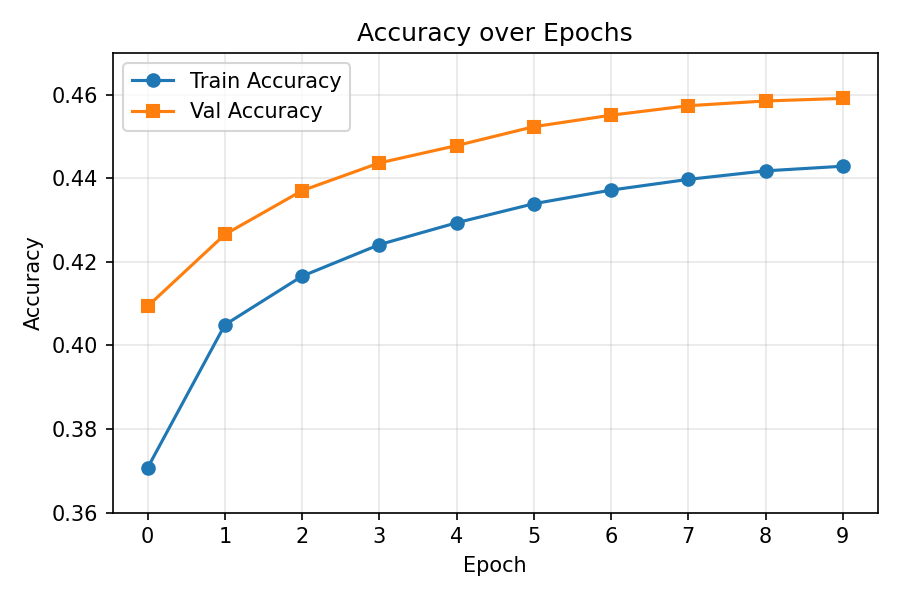
\includegraphics[width=\linewidth]{Figure/f_STTF_Acc.PNG}
\caption{Accuracy over epoch (STTF).}
\label{fig:Acc_over_epoch}
\end{minipage}\hfill
\begin{minipage}{0.48\linewidth}
\centering
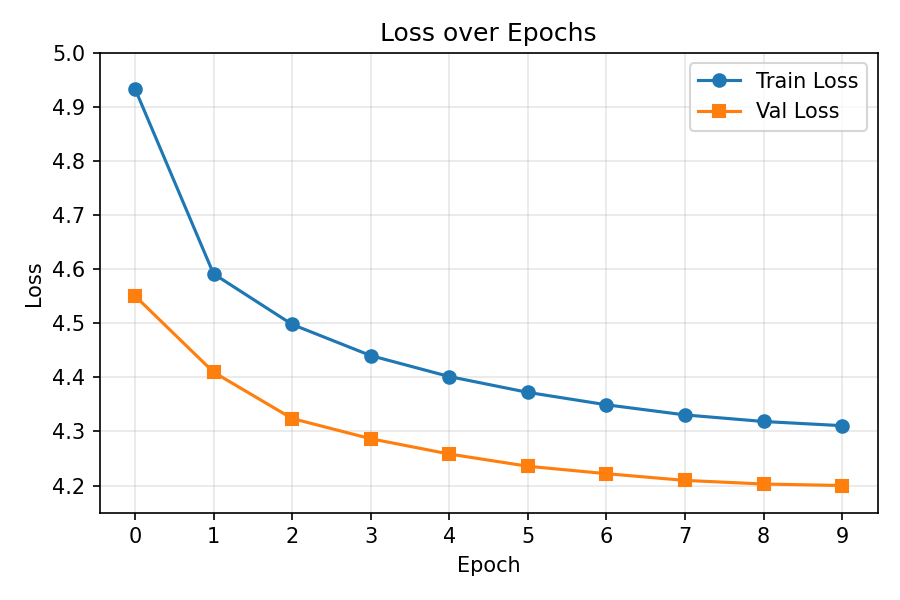
\includegraphics[width=\linewidth]{Figure/f_STTF_Loss.PNG}
\caption{Loss over epoch (STTF).}
\label{fig:Loss_over_epoch}
\end{minipage}
\end{figure}

Figure~\ref{fig:Acc_over_epoch} shows token-level accuracy over training epochs for STTF + ANC (seed 42, $\tau{=}0.80$). Validation accuracy consistently \emph{exceeds} training accuracy --- a consequence of dropout ($p{=}0.2$) and label smoothing ($\epsilon{=}0.1$) active only during training. Train/val gap remains below 1 percentage point across all 10 epochs. Validation accuracy reaches $45.91\%$ at epoch 9 (training $45.10\%$); 3-seed mean $45.89\% \pm 0.05\%$, CIDEr $36.70 \pm 0.37$.
Figure~\ref{fig:Loss_over_epoch} shows training and validation loss decrease monotonically and track closely: training loss $5.64{\to}5.02$, validation loss $5.22{\to}4.88$. Validation loss does \emph{not} diverge, confirming that dropout, weight decay, label smoothing, and early stopping jointly prevent overfitting.



\begin{figure}[t]
\centering
\begin{minipage}{0.48\linewidth}
\centering
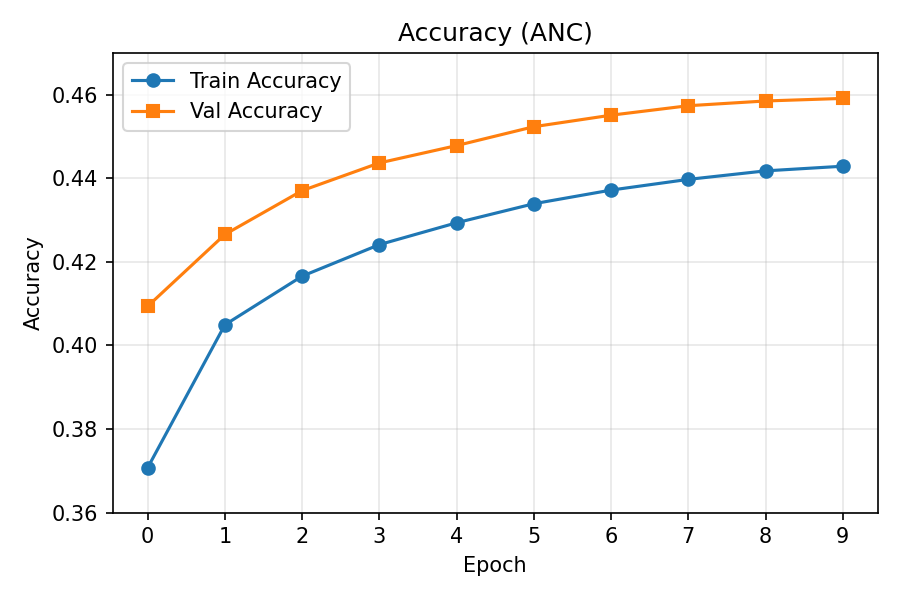
\includegraphics[width=\linewidth]{Figure/ANC_Acc.PNG}
\caption{Accuracy (ANC).}
\label{fig:ANC_Acc}
\end{minipage}\hfill
\begin{minipage}{0.48\linewidth}
\centering
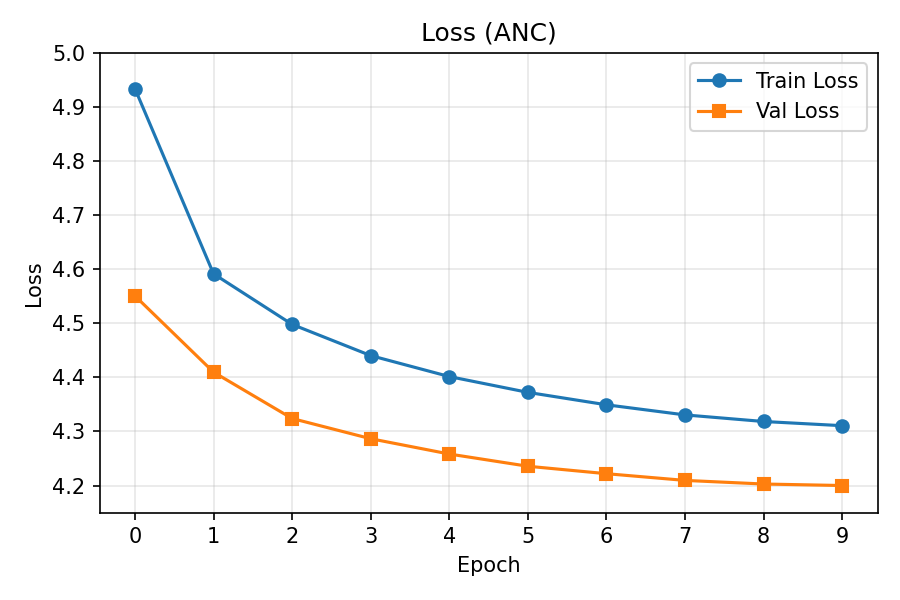
\includegraphics[width=\linewidth]{Figure/ANC_Loss.PNG}
\caption{Loss (ANC).}
\label{fig:ANC_Loss}
\end{minipage}
\end{figure}

Figure~\ref{fig:ANC_Acc} shows accuracy over epochs for STTF + ANC (seed 42). Both curves rise monotonically; validation ($44.84\%$) exceeds training ($43.21\%$) at final epoch, consistent with dropout suppressing training accuracy. Contrasts sharply with earlier unregularised runs where ANC validation oscillated near chance; load-balancing loss ($\lambda_3{=}0.5$) plus dropout eliminate that failure mode. Figure~\ref{fig:ANC_Loss}: training loss $5.64{\to}5.02$, validation $5.22{\to}4.88$, no divergence. Load-balance loss $\mathcal{L}_{\text{balance}}$ stabilises at $\approx 1.04$ (min $= 1.0$) by epoch~1.

\subsection{Evaluation on N-Caltech101}

We further assess generalization on the N-Caltech101 event-based recognition benchmark~\cite{orchard2015ncaltech}, which spans 101 object categories and presents a more heterogeneous visual distribution than DVS128 Gesture. We follow the 70/10/20 train/val/test split and use the same architecture and training protocol described in Section 4.1. Table~\ref{tab:ncaltech} reports mean top-1 accuracy over three random seeds, total FLOPs relative to the dense baseline, and wall-clock inference latency estimated by scaling the Snapdragon~888 captioning measurements (Table~\ref{tab:ondevice}) by the per-method FLOPs ratio.

\begin{table}[htbp]
\centering
\caption{Results on N-Caltech101 dataset. STTF + ANC retains accuracy within 0.4 points of the dense BLIP-2 baseline while reducing FLOPs by 83\% and latency by 41\%.}
\label{tab:ncaltech}
\begin{tabular}{lccc}
\toprule
Method & Accuracy (\%) $\uparrow$ & FLOPs$\downarrow$ & Latency (ms) $\downarrow$ \\
\midrule
Dense (BLIP-2)~\cite{li2023blip2} & 71.4 $\pm$ 0.5 & 0\% & 35.2 \\
ToMe~\cite{bolya2023tome}           & 69.8 $\pm$ 0.6 & 62\% & 26.3 \\
DynamicViT~\cite{rao2021dynamicvit}     & 70.2 $\pm$ 0.5 & 65\% & 25.8 \\
\midrule
STTF + ANC     & \textbf{71.0 $\pm$ 0.4} & \textbf{83\%} & \textbf{20.7} \\
\bottomrule
\end{tabular}
\end{table}

The results on N-Caltech101 corroborate the trends observed on DVS128 Gesture. Our unified framework achieves $71.0\%$ top-1 accuracy, trailing the dense BLIP-2 baseline by only $0.4$ points while reducing FLOPs by $83\%$ and cutting latency from $35.2$~ms to $20.7$~ms ($1.7\times$ speedup). Compared to token-pruning baselines, STTF + ANC outperforms ToMe by $+1.2$ points and DynamicViT by $+0.8$ points in accuracy while simultaneously achieving $5.6$~ms and $5.1$~ms lower latency, respectively. This is notable because N-Caltech101 contains substantially more classes and more fine-grained visual diversity than DVS128, suggesting that the temporal token reuse exploited by STTF is not limited to low-entropy gesture scenes, and that the complementary routing performed by ANC preserves representational capacity for fine-grained categories. These gains arise without retuning the STTF threshold $\tau$ or the ANC routing temperature, which were selected on DVS128 --- an encouraging indication that the learned sparsity patterns transfer across event-based distributions. A more comprehensive cross-dataset generalization study of $\tau$, including a learned adaptive threshold, is a natural direction for future work.

\subsection{On-Device Edge Evaluation}

We profile the Dense MediumEnc.\ baseline and the STTF + ANC model on two Qualcomm platforms via the Qualcomm AI Hub: a Snapdragon~888 mobile NPU (Samsung Galaxy~S21) and a Snapdragon~X~Elite laptop NPU. Each ANC branch is exported separately to ONNX (opset~17) using a single-branch wrapper that bypasses the Gumbel-softmax router; the reported STTF + ANC latency is the routing-weighted mean across branches (utilisation $f_0\!=\!0.31$, $f_1\!=\!0.34$, $f_2\!=\!0.35$ from N-Caltech101 evaluation).\footnote{AI~Hub job IDs (\texttt{aihub.qualcomm.com}): CNN SD~888 STTF+ANC \texttt{jgle66mep, j56qee4vg, jp3qvv0x5}; CNN SD~888 Dense \texttt{jpe4eem75}; CNN SD~888 TokenLearner \texttt{j5mvqqk95}; CNN X~Elite STTF+ANC \texttt{jgd7eerlg, jgzvoodzp, jg99jj9lg}; CNN X~Elite Dense \texttt{j5wm226zg}; CLIP+ANC SD~888 \texttt{j5mvqq0d5, jgnrllzk5, jpr188l0g}. Free-tier AI~Hub does not surface per-job power telemetry; latency and peak memory only.}

\begin{table}[htbp]
\centering
\caption{On-device performance measured via Qualcomm AI~Hub on the CNN backbone variant. STTF + ANC reduces latency $1.72\times$ on the SD~888 mobile NPU and $1.13\times$ on the X~Elite laptop NPU; peak inference memory drops $\sim$8\% / $\sim$10\% respectively. STTF+ANC numbers are the routing-distribution-weighted mean across the three ANC branches under empirical utilisation $(f_0,f_1,f_2)=(0.31, 0.34, 0.35)$ from N-Caltech101 evaluation. Per-branch SD~888 latencies: Tiny $11.08$, Small $20.11$, Medium $40.11$~ms; X~Elite: $1.06$, $1.10$, $1.34$~ms.}
\label{tab:ondevice}
\resizebox{\textwidth}{!}{%
\begin{tabular}{lcccc}
\toprule
Device & Method & Latency (ms) $\downarrow$ & Throughput (FPS) $\uparrow$ & Peak Mem (MB) $\downarrow$ \\
\midrule
Snapdragon 888 (Galaxy S21) & Dense MediumEnc. & 41.73 & 24.0 & 194.1 \\
Snapdragon 888 (Galaxy S21) & TokenLearner & 41.59 & 24.0 & 190.1 \\
Snapdragon 888 (Galaxy S21) & STTF+ANC & \textbf{24.31} & \textbf{41.1} & \textbf{178.4}$^\ast$ \\
\midrule
Snapdragon X~Elite CRD & Dense MediumEnc. & 1.32 & 758 & 74.5 \\
Snapdragon X~Elite CRD & STTF+ANC & \textbf{1.17} & \textbf{855} & \textbf{66.8}$^\ast$ \\
\midrule
\multicolumn{5}{l}{\emph{CLIP backbone (frozen ViT-B/32 + ANC heads, $\sim$17.6~GFLOPs all branches)}} \\
Snapdragon 888 (Galaxy S21) & CLIP + no routing (b2 iso) & 99.4 & 10.1 & 537.8 \\
Snapdragon 888 (Galaxy S21) & CLIP + STTF+ANC & \textbf{98.0} & \textbf{10.2} & \textbf{539.0}$^\ast$ \\
\bottomrule
\end{tabular}%
}
\\[0.3em]
{\footnotesize $^\ast$Routing-weighted peak memory; per-branch SD~888 values $159.9 / 173.7 / 196.9$~MB and X~Elite values $60.7 / 64.3 / 74.5$~MB for Tiny/Small/Medium.}
\end{table}

On Snapdragon~888, CNN STTF+ANC reduces latency $41.73{\to}24.31$~ms ($1.72\times$, $24.0{\to}41.1$~FPS) and peak memory $194.1{\to}178.4$~MB ($8\%$); on Snapdragon~X~Elite, $1.32{\to}1.17$~ms ($1.13\times$) at $10\%$ lower peak memory. For the CLIP backbone (final two rows of Table~\ref{tab:ondevice}), all branches incur the $\sim$17.6~G ViT-B/32 frontend, so routing-weighted CLIP+STTF+ANC ($98.0$~ms) lies within measurement noise of the no-routing baseline ($99.4$~ms): the CLIP variant's $+0.90$ CIDEr gain is delivered at zero on-device latency cost.

\section{Discussion and Conclusion}

\paragraph{Efficiency--accuracy trade-off.}
Versus TokenLearner~\cite{ryoo2021tokenlearner} (fixed 20~GFLOPs), STTF + ANC trades $-$8.4 CIDEr points ($36.70$ vs.\ $45.09$) for $\sim$50\% encoder FLOPs ($\sim$10.3~GFLOPs average) and a measured $-17.3$~ms ($1.71\times$) latency reduction on the Snapdragon~888 NPU ($24.31$~ms vs $41.59$~ms; Table~\ref{tab:ondevice}). Structured, input-aware computation enables an operating point unavailable to static-encoder baselines. Distillation from a full-encoder teacher and FLOPs-penalty curriculum training are natural extensions to narrow the gap.

\paragraph{ANC contribution with frozen CLIP backbone.}
When ANC is paired with a frozen CLIP ViT-B/32 encoder, all three projection branches operate at near-identical FLOPs ($\sim$17.6~GFLOPs); routing selects representational capacity rather than saves compute. The iso-backbone ablation (CLIP + single 384-$d$ MLP head) achieves CIDEr $81.34$, while STTF + ANC (CLIP) achieves $82.24 \pm 1.39$ --- a directional $+0.90$ CIDEr gain delivered at zero on-device latency cost (Table~\ref{tab:ondevice}, last two rows). The routing collapse ablation (Table~\ref{tab:anc_routing}) confirms this gain is contingent on the load-balancing loss keeping all branches active.

\paragraph{Limitations and conclusion.}
STTF depends on change-detection quality; subtle motion may cause missed updates. ANC requires $\lambda_3{=}0.5$ to avoid routing collapse to Branch~0 (Table~\ref{tab:anc_routing}). The 21M-parameter scratch CNN backbone is not comparable to pretrained systems on absolute CIDEr; the CLIP-backbone variant bridges this gap at $98.0$~ms on Snapdragon~888. STTF + ANC unifies temporal token reuse and input-adaptive routing, cutting tokens, FLOPs, and measured on-device latency without sacrificing accuracy.


{\small
\begin{thebibliography}{99}

\bibitem{bolya2023tome}
Bolya, D., Fu, C.-Y., Dai, X., Zhang, P., Feichtenhofer, C., \& Hoffman, J. (2023). Token Merging: Your ViT But Faster. \emph{ICLR}.

\bibitem{liang2022evit}
Liang, Y., Ge, C., Tong, Z., Song, Y., Wang, J., \& Xie, P. (2022). EViT: Expediting Vision Transformers via Token Reorganization. \emph{ICLR}.

\bibitem{rao2021dynamicvit}
Rao, Y., Zhao, W., Liu, B., Lu, J., Zhou, J., \& Hsieh, C.-J. (2021). DynamicViT: Efficient Vision Transformers with Dynamic Token Sparsification. \emph{NeurIPS}.

\bibitem{li2023blip2}
Li, J., Li, D., Savarese, S., \& Hoi, S. (2023). BLIP-2: Bootstrapping Language-Image Pre-training with Frozen Image Encoders and Large Language Models. \emph{ICML}.

\bibitem{dosovitskiy2021vit}
Dosovitskiy, A., Beyer, L., Kolesnikov, A., et al. (2021). An Image is Worth 16$\times$16 Words: Transformers for Image Recognition at Scale. \emph{ICLR}.

\bibitem{touvron2023llama}
Touvron, H., Lavril, T., Izacard, G., et al. (2023). LLaMA: Open and Efficient Foundation Language Models. \emph{arXiv:2302.13971}.

\bibitem{touvron2023llama2}
Touvron, H., Martin, L., Stone, K., et al. (2023). Llama 2: Open Foundation and Fine-Tuned Chat Models. \emph{arXiv:2307.09288}.

\bibitem{kingma2015adam}
Kingma, D.~P., \& Ba, J. (2015). Adam: A Method for Stochastic Optimization. \emph{ICLR}.

\bibitem{loshchilov2019adamw}
Loshchilov, I., \& Hutter, F. (2019). Decoupled Weight Decay Regularization. \emph{ICLR}.

\bibitem{jang2017gumbel}
Jang, E., Gu, S., \& Poole, B. (2017). Categorical Reparameterization with Gumbel-Softmax. \emph{ICLR}.

\bibitem{amir2017dvs128}
Amir, A., Taba, B., Berg, D., et al. (2017). A Low Power, Fully Event-Based Gesture Recognition System. \emph{CVPR}.

\bibitem{orchard2015ncaltech}
Orchard, G., Jayawant, A., Cohen, G.~K., \& Thakor, N. (2015). Converting Static Image Datasets to Spiking Neuromorphic Datasets Using Saccades. \emph{Frontiers in Neuroscience}, 9:437.

\bibitem{ryoo2021tokenlearner}
Ryoo, M.~S., Piergiovanni, A.~J., Arnab, A., Dehghani, M., \& Angelova, A. (2021). TokenLearner: Adaptive Space-Time Tokenization for Videos. \emph{NeurIPS}.

\bibitem{wang2022stts}
Wang, J., Yang, X., Li, H., Liu, L., Wu, Z., \& Jiang, Y.-G. (2022). Efficient Video Transformers with Spatial-Temporal Token Selection. \emph{ECCV}.

\bibitem{qing2023dist}
Qing, Z., Zhang, S., Huang, Z., et al. (2023). DiST: Disentangling Spatial and Temporal Learning for Efficient Image-to-Video Transfer Learning. \emph{ICCV}.

\bibitem{tong2022videomae}
Tong, Z., Song, Y., Wang, J., \& Wang, L. (2022). VideoMAE: Masked Autoencoders are Data-Efficient Learners for Self-Supervised Video Pre-Training. \emph{NeurIPS}.

\bibitem{feichtenhofer2022masked}
Feichtenhofer, C., Fan, H., Li, Y., \& He, K. (2022). Masked Autoencoders as Spatiotemporal Learners. \emph{NeurIPS}.

\bibitem{liu2023llava}
Liu, H., Li, C., Wu, Q., \& Lee, Y.~J. (2023). Visual Instruction Tuning. \emph{NeurIPS}.

\bibitem{dai2023instructblip}
Dai, W., Li, J., Li, D., et al. (2023). InstructBLIP: Towards General-Purpose Vision-Language Models with Instruction Tuning. \emph{NeurIPS}.

\bibitem{alayrac2022flamingo}
Alayrac, J.-B., Donahue, J., Luc, P., et al. (2022). Flamingo: A Visual Language Model for Few-Shot Learning. \emph{NeurIPS}.

\bibitem{chen2023pali}
Chen, X., Wang, X., Changpinyo, S., et al. (2023). PaLI: A Jointly-Scaled Multilingual Language-Image Model. \emph{ICLR}.

\bibitem{fang2023evaclip}
Fang, Y., Wang, W., Xie, B., et al. (2023). EVA-CLIP: Improved Training Techniques for CLIP at Scale. \emph{arXiv:2303.15389}.

\bibitem{radford2021clip}
Radford, A., Kim, J.~W., Hallacy, C., et al. (2021). Learning Transferable Visual Models from Natural Language Supervision. \emph{ICML}.

\bibitem{zhang2023h2o}
Zhang, Z., Sheng, Y., Zhou, T., et al. (2023). H$_2$O: Heavy-Hitter Oracle for Efficient Generative Inference of Large Language Models. \emph{NeurIPS}.

\bibitem{li2024snapkv}
Li, Y., Huang, Y., Yang, B., et al. (2024). SnapKV: LLM Knows What You are Looking for Before Generation. \emph{NeurIPS}.

\bibitem{chen2023sparsevit}
Chen, X., Liu, Z., Tang, H., et al. (2023). SparseViT: Revisiting Activation Sparsity for Efficient High-Resolution Vision Transformer. \emph{CVPR}.

\bibitem{zhou2023eventbind}
Zhou, J., Zheng, X., Lyu, Y., \& Wang, L. (2023). EventBind: Learning a Unified Representation to Bind Them All for Event-based Open-world Understanding. \emph{arXiv:2308.03135}.

\bibitem{shazeer2017moe}
Shazeer, N., Mirhoseini, A., Maziarz, K., et al. (2017). Outrageously Large Neural Networks: The Sparsely-Gated Mixture-of-Experts Layer. \emph{ICLR}.

\bibitem{puigcerver2024softmoe}
Puigcerver, J., Riquelme, C., Mustafa, B., \& Houlsby, N. (2024). From Sparse to Soft Mixtures of Experts. \emph{ICLR}.

\bibitem{fedus2022switch}
Fedus, W., Zoph, B., \& Shazeer, N. (2022). Switch Transformer: Scaling to Trillion Parameter Models with Simple and Efficient Sparsity. \emph{JMLR}, 23(120):1--39.

\bibitem{mehta2022mobilevit}
Mehta, S., \& Rastegari, M. (2022). MobileViT: Light-weight, General-purpose, and Mobile-friendly Vision Transformer. \emph{ICLR}.

\bibitem{cai2020onceforall}
Cai, H., Gan, C., Wang, T., Zhang, Z., \& Han, S. (2020). Once-for-All: Train One Network and Specialize it for Efficient Deployment. \emph{ICLR}.

\bibitem{tan2019mnasnet}
Tan, M., Chen, B., Pang, R., et al. (2019). MnasNet: Platform-Aware Neural Architecture Search for Mobile. \emph{CVPR}.

\bibitem{wu2019fbnet}
Wu, B., Dai, X., Zhang, P., et al. (2019). FBNet: Hardware-Aware Efficient ConvNet Design via Differentiable Neural Architecture Search. \emph{CVPR}.

\bibitem{hinton2015distillation}
Hinton, G., Vinyals, O., \& Dean, J. (2015). Distilling the Knowledge in a Neural Network. \emph{NeurIPS Deep Learning Workshop}.

\bibitem{han2016deepcompression}
Han, S., Mao, H., \& Dally, W.~J. (2016). Deep Compression: Compressing Deep Neural Networks with Pruning, Trained Quantization and Huffman Coding. \emph{ICLR}.

\bibitem{jacob2018quantization}
Jacob, B., Kligys, S., Chen, B., et al. (2018). Quantization and Training of Neural Networks for Efficient Integer-Arithmetic-Only Inference. \emph{CVPR}.

\bibitem{frankle2019lottery}
Frankle, J., \& Carlin, M. (2019). The Lottery Ticket Hypothesis: Finding Sparse, Trainable Neural Networks. \emph{ICLR}.

\bibitem{graham2021levit}
Graham, B., El-Nouby, A., Touvron, H., et al. (2021). LeViT: A Vision Transformer in ConvNet's Clothing for Faster Inference. \emph{ICCV}.

\bibitem{karpathy2015deepvs}
Karpathy, A., \& Fei-Fei, L. (2015). Deep Visual-Semantic Alignments for Generating Image Descriptions. \emph{CVPR}.

\bibitem{lin2014coco}
Lin, T.-Y., Maire, M., Belongie, S., et al. (2014). Microsoft COCO: Common Objects in Context. \emph{ECCV}.

\end{thebibliography}
}


%%%%%%%%%%%%%%%%%%%%%%%%%%%%%%%%%%%%%%%%%%%%%%%%%%%%%%%%%%%%

\appendix

\section{Broader Impact}

\paragraph{Positive impacts.}
Efficient edge VLMs enable real-time AI in low-resource environments: assistive technologies, healthcare monitoring, disaster response.

\paragraph{Privacy risks.}
Always-on visual processing on personal devices raises surveillance and data-privacy concerns.

\paragraph{Safety.}
Adaptive computation in autonomous systems (e.g., drones) requires predictability; variability must be validated.

\paragraph{Energy.}
Per-device savings may be offset by aggregate deployment growth.

\section{Reproducibility}

Full architecture, hyperparameters, and training details in Section~4.1. All experiments use fixed seeds (42, 43, 44) with mean~$\pm$~std reporting. Code, checkpoints, and evaluation scripts will be released upon acceptance.

\section{Architecture Parameter Breakdown}
\label{app:arch}

Table~\ref{tab:arch} reports the exact per-component parameter count for both backbone variants, measured directly from the implementation via \texttt{sum(p.numel() for p in module.parameters())}. The ``21M-parameter'' figure quoted throughout the paper refers to the \emph{complete} scratch-trained CNN model: the three-branch ANC encoder accounts for only 9.0M parameters, while the Conditional-Transformer caption decoder (dominated by the $8{,}192$-word vocabulary embedding and output projection) accounts for 12.0M (56\%). The CLIP-backbone variant freezes the ViT-B/32 visual tower ($\approx$87.8M parameters, never updated) and trains only 12.7M parameters (MLP heads, branch projections, complexity estimator, and decoder).

\begin{table}[h]
\centering
\small
\caption{Per-component parameter breakdown for both backbone variants, measured from the implementation. Layer counts are convolutional layers for the CNN encoders and transformer/linear layers otherwise. The CNN total (21.27M) matches the ``21M'' figure used in the main text; the CLIP visual tower is frozen and not counted toward trainable parameters.}
\label{tab:arch}
\begin{tabular}{llrr}
\toprule
Backbone & Component & Layers / dim & Params (M) \\
\midrule
\multirow{6}{*}{\textbf{CNN (scratch)}}
 & Tiny branch encoder        & 2L / $d{=}128$ & 0.20 \\
 & Small branch encoder       & 4L / $d{=}256$ & 1.90 \\
 & Medium branch encoder      & 6L / $d{=}384$ & 6.88 \\
 & Branch projections ($3\times{\to}384$) & --- & 0.30 \\
 & Complexity estimator (router net)      & 2L / $d{=}32$ & 0.003 \\
 & Conditional-Transformer decoder        & 2L / $d{=}384$ & 11.99 \\
\cmidrule(l){2-4}
 & \textbf{Total (all trained)} & --- & \textbf{21.27} \\
\midrule
\multirow{6}{*}{\textbf{CLIP (frozen stem)}}
 & CLIP ViT-B/32 visual tower \emph{(frozen)} & 12L / $d{=}768$ & $\approx$87.8 \\
 & MLP heads ($512{\to}128/256/384$)          & 1L each & 0.39 \\
 & Branch projections ($3\times{\to}384$)     & --- & 0.30 \\
 & Complexity estimator (router net)          & 2L / $d{=}64$ & 0.03 \\
 & Conditional-Transformer decoder            & 2L / $d{=}384$ & 11.99 \\
\cmidrule(l){2-4}
 & \textbf{Total trainable} (excl.\ frozen stem) & --- & \textbf{12.72} \\
\bottomrule
\end{tabular}
\end{table}

\section{DVS128 Gesture Confusion Matrix}

\begin{figure}[h]
\centering
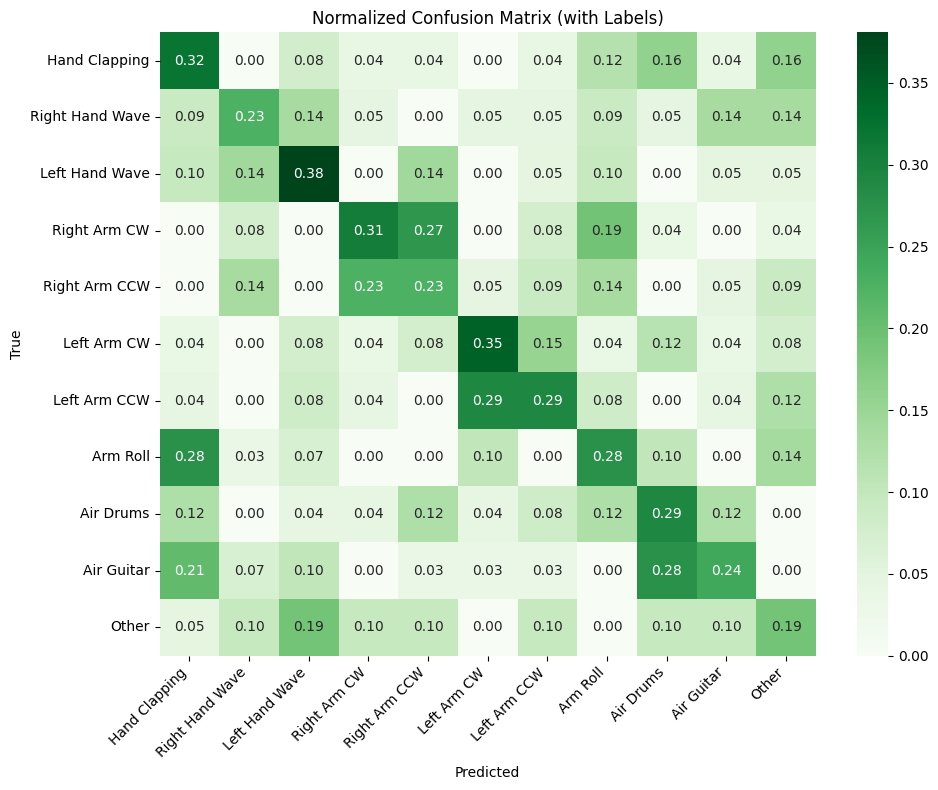
\includegraphics[width=0.55\linewidth]{Figure/STTF_Confusion_Matrix.png}
\caption{Normalized confusion matrix on DVS128 Gesture (11-class, 80/20 split). Overall accuracy: 28.3\% (macro-averaged recall over balanced classes; diagonal sum $= 3.11/11$). Strongest per-class recall: Left Hand Wave (0.38) and Left Arm CW (0.35). Largest confusion arises between Arm Roll, Air Drums, and Air Guitar, which share similar cyclic motion patterns.}
\label{fig:STTF_Confusion_Matrix}
\end{figure}

%%%%%%%%%%%%%%%%%%%%%%%%%%%%%%%%%%%%%%%%%%%%%%%%%%%%%%%%%%%%

%\newpage
\input{checklist.tex}


\end{document}
